\begin{figure}[H]
    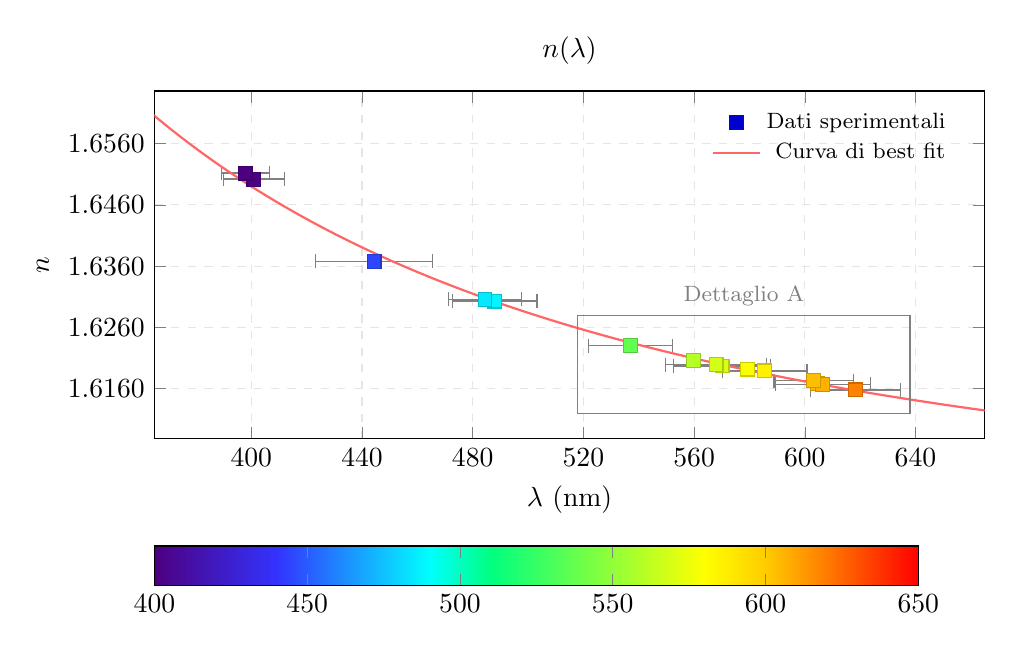
\begin{tikzpicture}
        \begin{axis}[
            title={\(n(\lambda)\)},
            width=\linewidth,
            height=6cm,
            xlabel={\(\lambda\) (nm)},
            ylabel={\(n\)},
            grid=both,
            grid style={dashed, gray!20},
            ytick={1.6160,1.6260,1.6360,1.6460,1.6560},
            yticklabels={1.6160,1.6260,1.6360,1.6460,1.6560},
            xtick={400, 440, 480, 520,560, 600, 640},
            xticklabels={400, 440, 480, 520,560, 600, 640},
            xmin=365, xmax=665,
            legend pos=north east,
            legend style={
                draw=none,
                fill=none,
                text opacity=1,
                font=\footnotesize,
                cells={anchor=east}
            },
            colormap={visiblespectrum}{
                rgb(400)=(0.3,0,0.5)   % violet (corrected wavelength)
                rgb(440)=(0.2,0.2,1)   % blue
                rgb(490)=(0,1,1)     % cyan
                rgb(510)=(0,1,0.5)   % green
                rgb(580)=(1,1,0)     % yellow
                rgb(600)=(1,0.8,0)   % orange
                rgb(650)=(1,0,0)     % red
            },
            point meta min=400,
            point meta max=650
            ]

            % Dati principali con colori dello spettro
            \addplot+ [
            scatter,
            only marks,
            mark=square*,
            scatter src=x,
            mark size=2.5,
            visualization depends on={\thisrow{yerr}\as\perror},
            visualization depends on={\thisrow{xerr}\as\xerror},
            error bars/.cd,
            x dir=both, x explicit,
            y dir=both, y explicit,
            error bar style={line width=0.5pt, solid, black!50}
            ] table [
            x=x,
            y=y,
            x error=xerr,
            y error=yerr,
            ] {
                y     yerr   x       xerr
                1.6168  0.0002  604.59  1.91
                1.6192  0.0002  579.42  1.10
                1.6206  0.0002  559.67  2.05
                1.6158  0.0002  618.41  16.20
                1.6167  0.0002  606.50  17.16
                1.6173  0.0002  603.16  14.30
                1.6189  0.0002  585.51  15.27
                1.6197  0.0002  570.11  17.54
                1.6199  0.0002  567.93  18.37
                1.6230  0.0002  537.14  15.16
                1.6303  0.0002  487.91  15.31
                1.6306  0.0002  484.43  13.30
                1.6368  0.0002  444.34  21.02
                1.6502  0.0002  400.94  11.05
                1.6512  0.0002  397.91  8.61
            };
            \addlegendentry{Dati sperimentali}

            \addplot[
            red!60,
            thick,
            domain=340:750,
            samples=200
            ] {
                1.591703 + 9.171e3/x^2
            };
            \addlegendentry{Curva di best fit}

            \draw[gray]
            (axis cs:518,1.612) rectangle
            (axis cs:638,1.628);

            \node[gray,above, align=center, font=\footnotesize] at (axis cs:578,1.628)
            {Dettaglio A};

            % Barra dei colori con spettro visibile
            \pgfplotsset{
                colorbar horizontal,
                colorbar style={
                    xtick={400,450,500,550,600,650},
                    width=0.8\linewidth,
                    xlabel style={yshift=-0.5cm},
                    colormap name=visiblespectrum
                }
            }
        \end{axis}
    \end{tikzpicture}
    \centering
    \caption{Unione dei dati ricavati con la lampada al sodio e di quelli ricavati con la lampada al mercurio. I punti sono colorati secondo lo spettro visibile corrispondente alla loro lunghezza d'onda, da 400 nm (viola) a 650 nm (rosso). La regione delimitata (Dettaglio A) verrà analizzata separatamente nella figura successiva.}
\end{figure}